
\documentclass{sig-alternate-05-2015}
% Pages are numbered in submission mode, and unnumbered in camera-ready
\usepackage{subfigure}
\usepackage{ctex}
\usepackage{graphicx}
\usepackage{times}
\usepackage{epsfig}
%\usepackage{figure}

\usepackage{amsmath}
\usepackage{amssymb}
% Pages are numbered in submission mode, and unnumbered in camera-ready
\begin{document}
\setcopyright{acmcopyright}

%%%%%%%%% TITLE
\title{近代以来中华民族观念的形成与演变}

\author{
	% You can go ahead and credit any number of authors here,
	% e.g. one 'row of three' or two rows (consisting of one row of three
	% and a second row of one, two or three).
	%
	% The command \alignauthor (no curly braces needed) should
	% precede each author name, affiliation/snail-mail address and
	% e-mail address. Additionally, tag each line of
	% affiliation/address with \affaddr, and tag the
	% e-mail address with \email.
	%
	% 1st. author
	\alignauthor
	Yue Wu\titlenote\\
	王梦迪\titlenote\\
	\email{1600012704@pku.edu.cn}
}

\maketitle
%\thispagestyle{empty}


%%%%%%%%% ABSTRACT


%%%%%%%%% BODY TEXT
\section{简介}

%    \begin{figure}
%		\begin{center}
%		\subfigure{
%		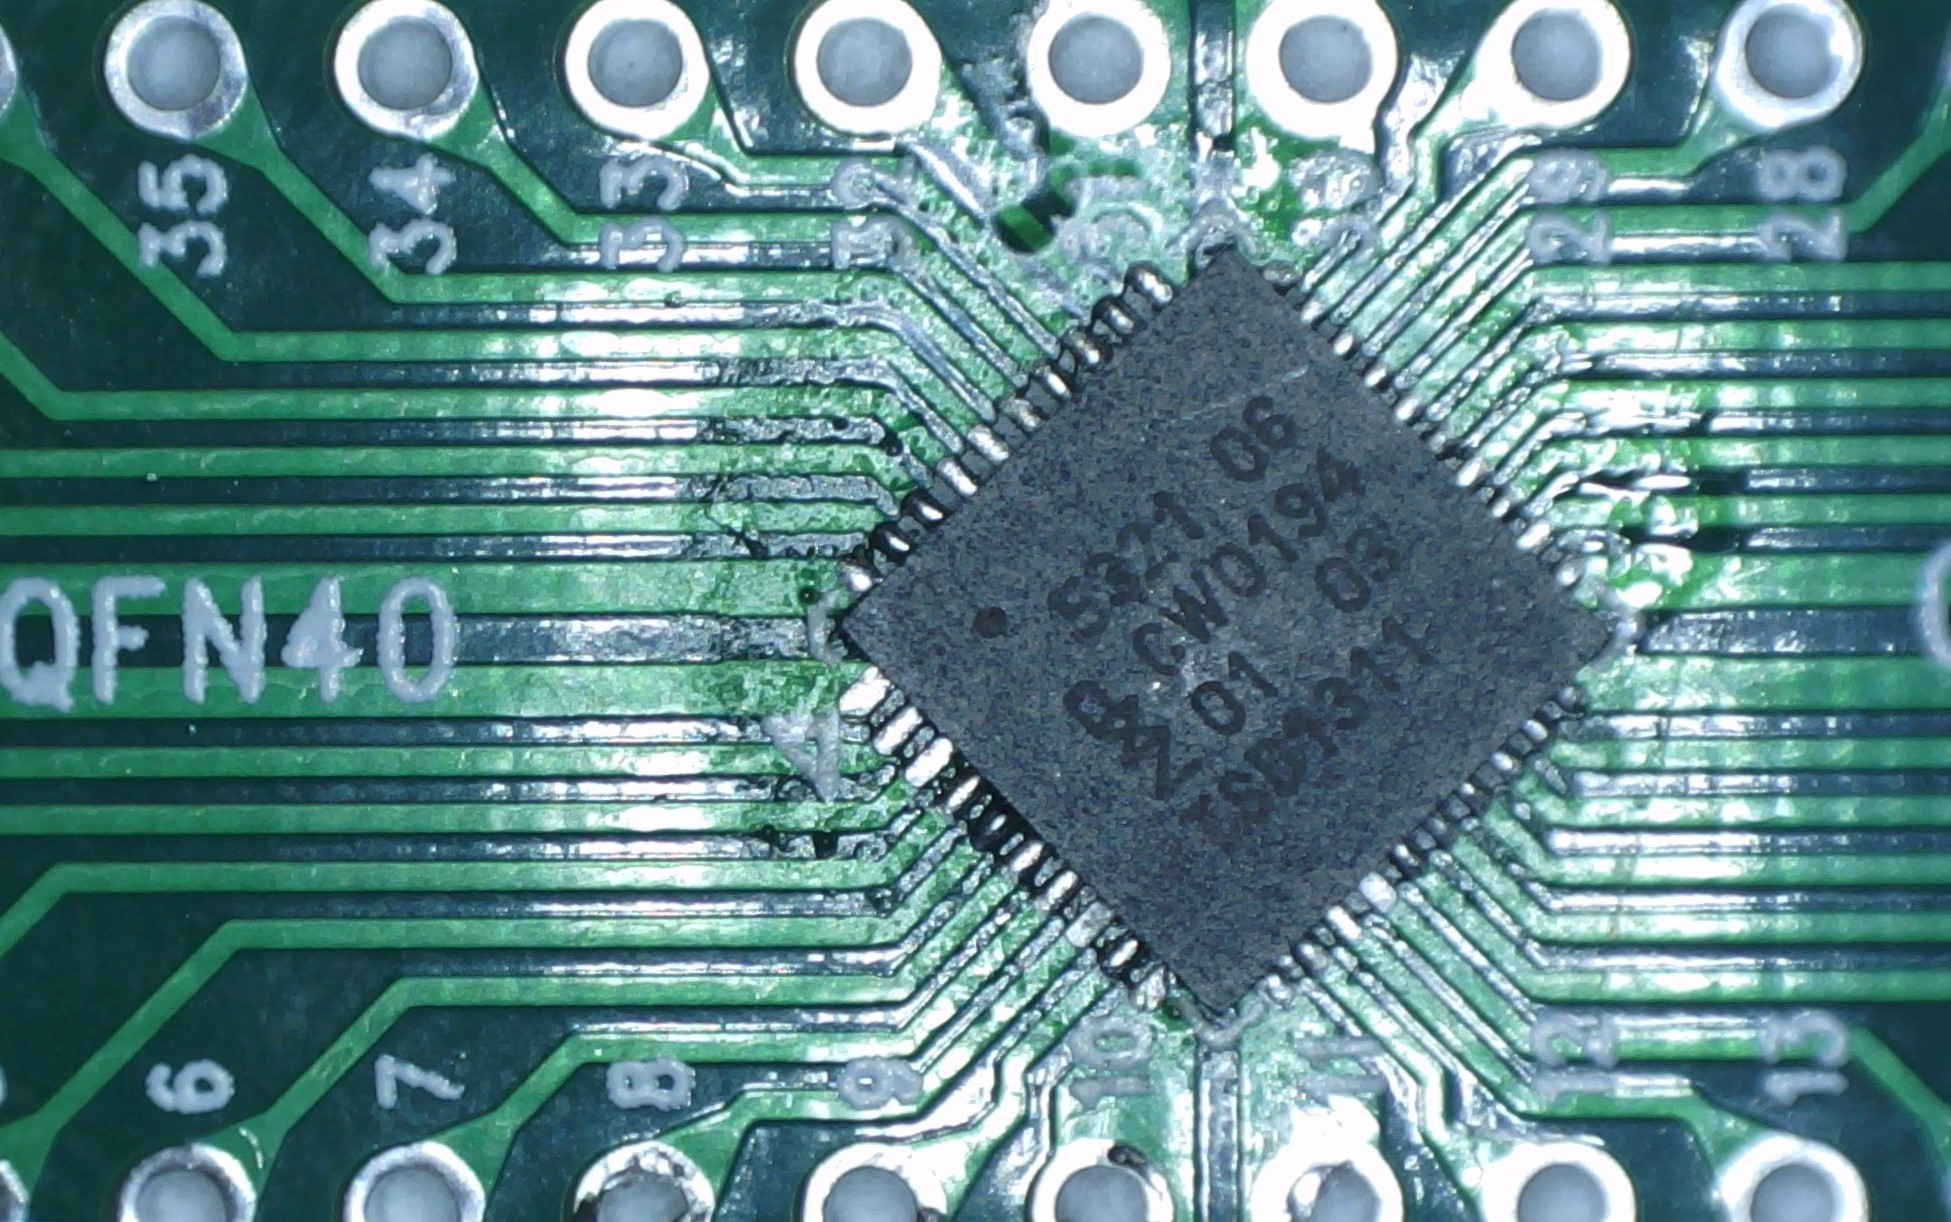
\includegraphics[scale = 0.15]{PN532}
%		}
%		\end{center}
%		\caption{PN532}
%	\end{figure}
	中华民族形成很早,但并没有形成现代意义上的民族主义,中国古人持“华夷之辨”,以文化而非血缘传统来判定一个人的归属。自1840年鸦片战争后,帝国主义用枪炮打开了中国的大门,让中华民族面临前所未有的危机。与此同时,西方的科学、文化也开始传入中国,其中就包括西方民族主义,这促进了中国本土民族主义的发展,而中国本土的民族主义导致了中华民族意识的觉醒,将中华民族凝结成一个统一的民族共同体,向一个现代的民族国家进行转变。


\section{清末民初的中华民族观念}

\subsection{梁启超}
梁启超是最早引进西方民族主义,并在此基础上提出和使用“中华民族”这一观念的人。1901年,梁启超发表了在《中国史叙论》一文。梁启超在文中称,“吾人所最惭愧者。莫如我国无国名之一事。寻常通称。或曰诸夏。或曰汉人。或曰唐人。皆朝名也。外人所称。或曰震旦。或曰支那。皆非我所自命之名也。”可见古代中国人并没有明确地对自己的民族进行定义,只是模糊地进行代称。文中提出了“中国民族”这一说法,将中华民族这一传统上的文化观念视为一个近代意义上的民族。文中将中国民族的演变历史划分为三个时代:“第一,上世史,自黄帝以迄秦之一统,是为中国之中国,即中国民族自发达、自竞争、自团结之时代也”;“第二,中世史,自秦统一后至清代乾隆之末年,是为亚洲之中国,即中国民族与亚洲各民族交涉、繁赜、竞争最激烈之时代也”;“第三,近世史,自乾隆末年以至于今日,是为世界之中国,即中国民族合同全亚洲民族与西人交涉、竞争之时代也”。
%%CITE HERE

1902年,梁启超在《中国学术思想变迁之大势》中,论述战国时期齐国的学术思想时提出:“齐,海国也。上古时代,我中华民族之有海思想者厥惟齐。故于其间产出两种观念焉:一曰国家观,二曰世界观。”在该文中,梁启超对“中华”的内涵做了说明:“立于五洲中之最大洲而为其洲中之最大国者,谁乎?我中华也;人口之居全地球三分之一者,谁乎?我中华也;四千余年之历史未尝一基础中断者,谁乎?我中华也。我中华有四百兆人公用之语言文字,世界莫能及。我中华有三十世纪前传以来之古书,世界莫能及。”
%%CITE HERE

1905年,梁启超在《历史上中国民族之观察》一文中,使用了“中华民族”七次(简称为“华族”),并明确表示:“今之中华民族,即普遍俗称所谓汉族者”,它是“我中国主族,即所谓炎黄遗族。”,由此可知梁启超主张中华民族就等于汉族,他将中华民族认定为汉族与其前身华夏族,这与今日的定义,即中华民族指中国境内的所有民族,中国是一个统一的多民族国家不同。

梁启超为晚清君主立宪的改革派人士代表,反对鼓吹推翻满清建立共和的革命党政治主张,主张将满清疆域境内各民族视为一个整体来拯救的“大民族主义”。梁启超将革命党政治主张描述成对立的“小民族主义”,认为“小民族主义”鼓吹汉族独立建国,从满清的统治中独立复兴单一民族。

\subsection{杨度}
继梁启超之后,晚清著名立宪派代表杨度也成为“中华民族”一词的早期使用者。杨度在1907年发表的《金铁主义说》一文中不仅多次提到“中华民族”,并且还比较清楚地说明了“中华”作为民族名称的由来和特征:“中国向来虽无民族二字之名词,实有何等民族之称号。今人必目中国最旧之民族曰汉民族,其实汉为刘家天子时代之朝号,而非其民族之名也。中国自古有一文化较高、人数较多之民族在其国中,自命其国曰中国,自命其民族曰中华。即此义以求之,则一国家与一国家之别,别于地域,中国云者,以中外别地域远近也。一民族与一民族之别,别于文化,中华云者,以华夷别文化之高下也。”
%%CITE HERE

杨度主张“汉”只是“刘家天子时代之朝号”,应采“中华”为“文化之族名”以反对“汉族”血统说。因此杨度 也成为了中华民族一词的早期使用者,但其强调以中国自古以来以“文化较高、人数较多”的历史文化定义和梁启超的政治文化定义有所不同。杨度提倡中华民族为中华文化之族名,将中国全体人民尽成为中华民族。





\section{Paper Reading}

	\subsection{Intensive}
		\cite{SWless}
		\cite{SurNfc}
		\cite{WTraMag}
		\cite{magP}
		\cite{pocketC}
		\cite{wirelessALL}
	\subsection{extensive}
        \cite{6176332}
        \cite{6838830}
        \cite{7056164}
        \cite{6902086}
        \cite{Fei:2013:PPP:2512349.2514593}
        \cite{7428884}
        \cite{4782856}
	
{\small
	\bibliographystyle{ieee}
	\bibliography{SGbib}
}

\end{document}
